\subsection{Scenario 2: Risk Introduction}
\label{ssec:scenario-2-results}
\textit{This scenario introduces a risk to the infrastructure after $180$ seconds. The purpose of this scenario is to see how the system behaves when a new risk is introduced.}

\begin{figure}[H]
    \centering
    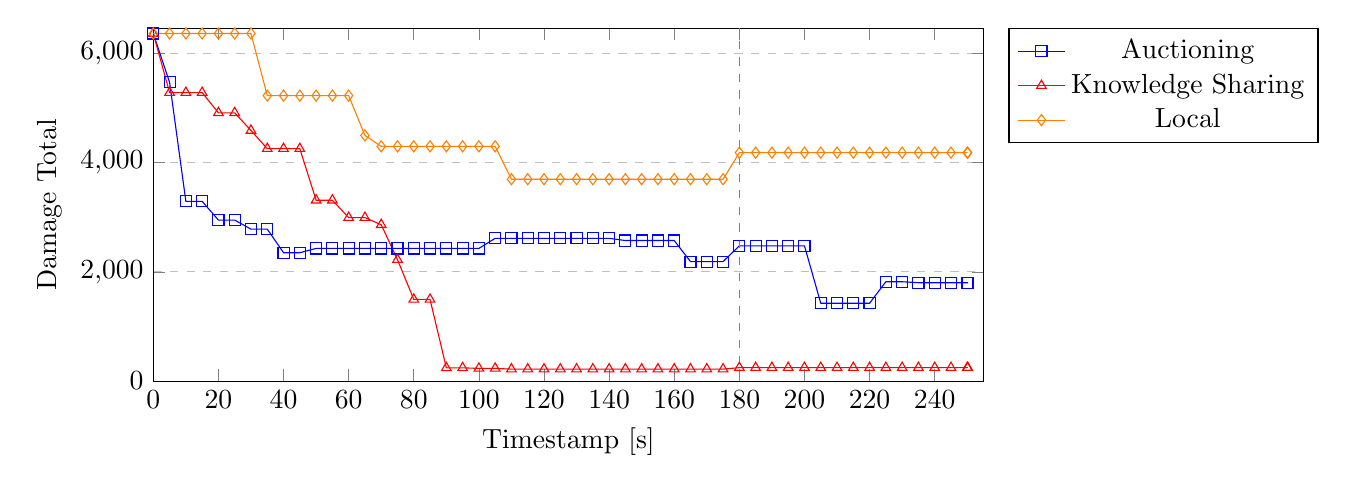
\begin{tikzpicture}
\begin{axis}[
    xlabel={Timestamp [s]},
    ylabel={Damage Total},
    xmin=0, xmax=255000,
    ymin=0, ymax=6464,
    legend pos=outer north east,
    ymajorgrids=true,
    grid style=dashed,
    width=\textwidth,
    height=0.5\textwidth,
    scaled x ticks=base 10:-3,
    xtick scale label code/.code={}
]

	\addplot[color=blue,mark=square] coordinates {
        (0,6367.26)(5000,5473.92)(10000,3293.02)(15000,3293.02)(20000,2949.34)(25000,2949.34)(30000,2783.36)(35000,2783.36)(40000,2351.49)(45000,2351.49)(50000,2430.01)(55000,2430.01)(60000,2430.01)(65000,2430.01)(70000,2430.01)(75000,2430.01)(80000,2430.01)(85000,2430.01)(90000,2430.01)(95000,2430.01)(100000,2430.01)(105000,2615.26)(110000,2615.26)(115000,2615.26)(120000,2615.26)(125000,2615.26)(130000,2615.26)(135000,2615.26)(140000,2615.26)(145000,2574.45)(150000,2574.45)(155000,2574.45)(160000,2574.45)(165000,2188.56)(170000,2188.56)(175000,2188.56)(180000,2477.58)(185000,2477.58)(190000,2477.58)(195000,2477.58)(200000,2477.58)(205000,1426.19)(210000,1426.19)(215000,1426.19)(220000,1426.19)(225000,1819.63)(230000,1819.63)(235000,1802.13)(240000,1802.13)(245000,1802.13)(250000,1802.13)(250288,1802.13)
    };
    \addlegendentry{Auctioning}
	\addplot[color=red,mark=triangle] coordinates {
        (0,6367.26)(5000,5284.52)(10000,5284.52)(15000,5284.52)(20000,4914.13)(25000,4914.13)(30000,4590.69)(35000,4257.62)(40000,4257.62)(45000,4257.62)(50000,3313.54)(55000,3313.54)(60000,2994.50)(65000,2994.50)(70000,2864.46)(75000,2224.62)(80000,1496.52)(85000,1496.52)(90000,242.72)(95000,242.72)(100000,232.18)(105000,232.18)(110000,219.25)(115000,219.25)(120000,219.25)(125000,219.25)(130000,219.25)(135000,219.25)(140000,219.25)(145000,219.25)(150000,219.25)(155000,219.25)(160000,219.25)(165000,219.25)(170000,219.25)(175000,219.25)(180000,245.68)(185000,245.68)(190000,245.68)(195000,245.68)(200000,245.68)(205000,245.68)(210000,245.68)(215000,245.68)(220000,245.68)(225000,245.68)(230000,245.68)(235000,245.68)(240000,245.68)(245000,245.68)(250000,245.68)(250159,245.68)
    };
    \addlegendentry{Knowledge Sharing}
	\addplot[color=orange,mark=diamond] coordinates {
        (0,6367.26)(5000,6367.26)(10000,6367.26)(15000,6367.26)(20000,6367.26)(25000,6367.26)(30000,6367.26)(35000,5229.23)(40000,5229.23)(45000,5229.23)(50000,5229.23)(55000,5229.23)(60000,5229.23)(65000,4499.97)(70000,4300.22)(75000,4300.22)(80000,4300.22)(85000,4300.22)(90000,4300.22)(95000,4300.22)(100000,4300.22)(105000,4300.22)(110000,3698.17)(115000,3698.17)(120000,3698.17)(125000,3698.17)(130000,3698.17)(135000,3698.17)(140000,3698.17)(145000,3698.17)(150000,3698.17)(155000,3698.17)(160000,3698.17)(165000,3698.17)(170000,3698.17)(175000,3698.17)(180000,4184.36)(185000,4184.36)(190000,4184.36)(195000,4184.36)(200000,4184.36)(205000,4184.36)(210000,4184.36)(215000,4184.36)(220000,4184.36)(225000,4184.36)(230000,4184.36)(235000,4184.36)(240000,4184.36)(245000,4184.36)(250000,4184.36)(250135,4184.36)
    };
    \addlegendentry{Local}

	\addplot[color=gray, dashed,] coordinates {(180000,0) (180000,6464)};


\end{axis}
\end{tikzpicture}
    \caption{This graph shows the overall damage of the system in the risk introduction scenario. The damage is shown for each of the three strategies. The vertical lines indicate the time at which a risk is introduced.}
    \label{fig:overall-damage-inroduce-risk}
\end{figure}

Figure \ref{fig:overall-damage-inroduce-risk} shows a graph that follows a similar trend as shown in Figure \ref{fig:overall-damage-no-change}, albeit a bit slower for the auctioning agent. This is to be expected as the scenarios are identical up until the $120$ seconds mark. During this time we see a small increase in damage for all graphs. As the metrics are collected in $5000$ms intervals, we see a small bump in all the lines around the $120$ seconds mark. And it slowly goes down again after this. Due to this timing, agents sometimes applied the adaptation before the interval ended. This explains why sometimes the lines are not as smooth as we would expect.

\begin{figure}[H]
    \centering
    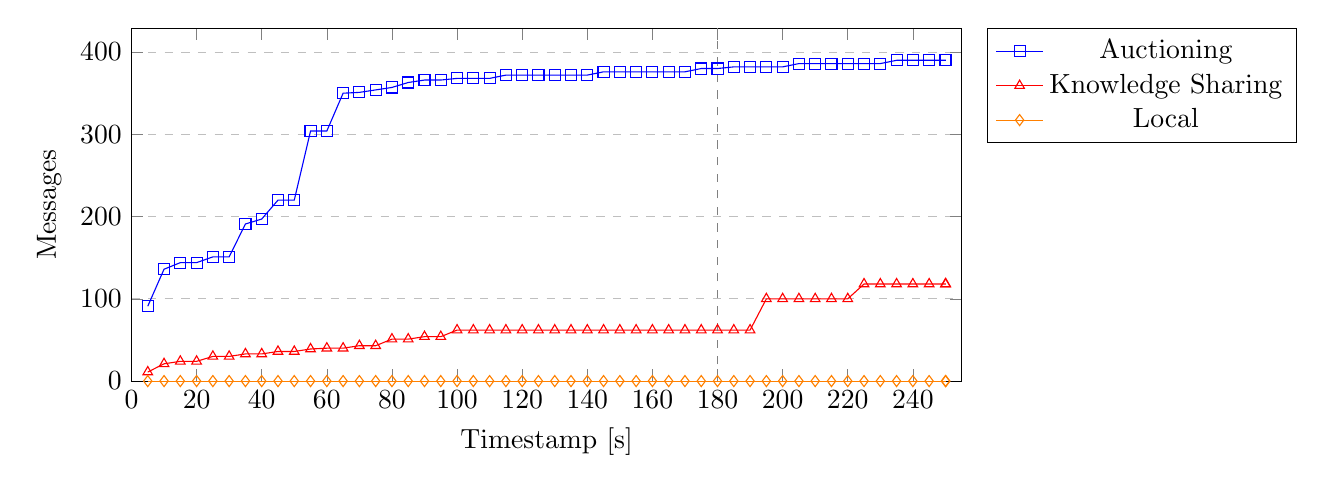
\begin{tikzpicture}
\begin{axis}[
    xlabel={Timestamp [s]},
    ylabel={Messages},
    xmin=0, xmax=255000,
    ymin=0, ymax=429,
    legend pos=outer north east,
    ymajorgrids=true,
    grid style=dashed,
    width=\textwidth,
    height=0.5\textwidth,
    scaled x ticks=base 10:-3,
    xtick scale label code/.code={}
]

	\addplot[color=blue,mark=square] coordinates {
        (5000,91)(10000,136)(15000,144)(20000,144)(25000,151)(30000,151)(35000,191)(40000,197)(45000,220)(50000,220)(55000,304)(60000,304)(65000,350)(70000,351)(75000,354)(80000,357)(85000,363)(90000,366)(95000,366)(100000,368)(105000,368)(110000,368)(115000,372)(120000,372)(125000,372)(130000,372)(135000,372)(140000,372)(145000,376)(150000,376)(155000,376)(160000,376)(165000,376)(170000,376)(175000,380)(180000,380)(185000,382)(190000,382)(195000,382)(200000,382)(205000,386)(210000,386)(215000,386)(220000,386)(225000,386)(230000,386)(235000,390)(240000,390)(245000,390)(250000,390)(250139,390)
    };
    \addlegendentry{Auctioning}
	\addplot[color=red,mark=triangle] coordinates {
        (5000,11)(10000,21)(15000,24)(20000,24)(25000,30)(30000,30)(35000,33)(40000,33)(45000,36)(50000,36)(55000,39)(60000,40)(65000,40)(70000,43)(75000,43)(80000,51)(85000,51)(90000,54)(95000,54)(100000,62)(105000,62)(110000,62)(115000,62)(120000,62)(125000,62)(130000,62)(135000,62)(140000,62)(145000,62)(150000,62)(155000,62)(160000,62)(165000,62)(170000,62)(175000,62)(180000,62)(185000,62)(190000,62)(195000,100)(200000,100)(205000,100)(210000,100)(215000,100)(220000,100)(225000,118)(230000,118)(235000,118)(240000,118)(245000,118)(250000,118)(250111,118)
    };
    \addlegendentry{Knowledge Sharing}
	\addplot[color=orange,mark=diamond] coordinates {
        (5000,0)(10000,0)(15000,0)(20000,0)(25000,0)(30000,0)(35000,0)(40000,0)(45000,0)(50000,0)(55000,0)(60000,0)(65000,0)(70000,0)(75000,0)(80000,0)(85000,0)(90000,0)(95000,0)(100000,0)(105000,0)(110000,0)(115000,0)(120000,0)(125000,0)(130000,0)(135000,0)(140000,0)(145000,0)(150000,0)(155000,0)(160000,0)(165000,0)(170000,0)(175000,0)(180000,0)(185000,0)(190000,0)(195000,0)(200000,0)(205000,0)(210000,0)(215000,0)(220000,0)(225000,0)(230000,0)(235000,0)(240000,0)(245000,0)(250000,0)(250115,0)
    };
    \addlegendentry{Local}

	\addplot[color=gray, dashed,] coordinates {(180000,0) (180000,429)};


\end{axis}
\end{tikzpicture}
    \caption{Graph showing the total amount of messages sent between agents in the risk introduction scenario.}
    \label{fig:messages-risk-introduction}
\end{figure}

Figure \ref{fig:messages-risk-introduction} shows a graph similar to Figure \ref{fig:messages-no-change}. The auctioning agent sends the most messages, followed by the knowledge-sharing agent. The local-agent sends no messages. We see that after the $120$ seconds mark, both the auctioning and knowledge-sharing agents send a few more messages around. This is to be expected as the agents detect a change in their properties, and start sharing this information with other agents.

\begin{figure}[H]
    \centering
    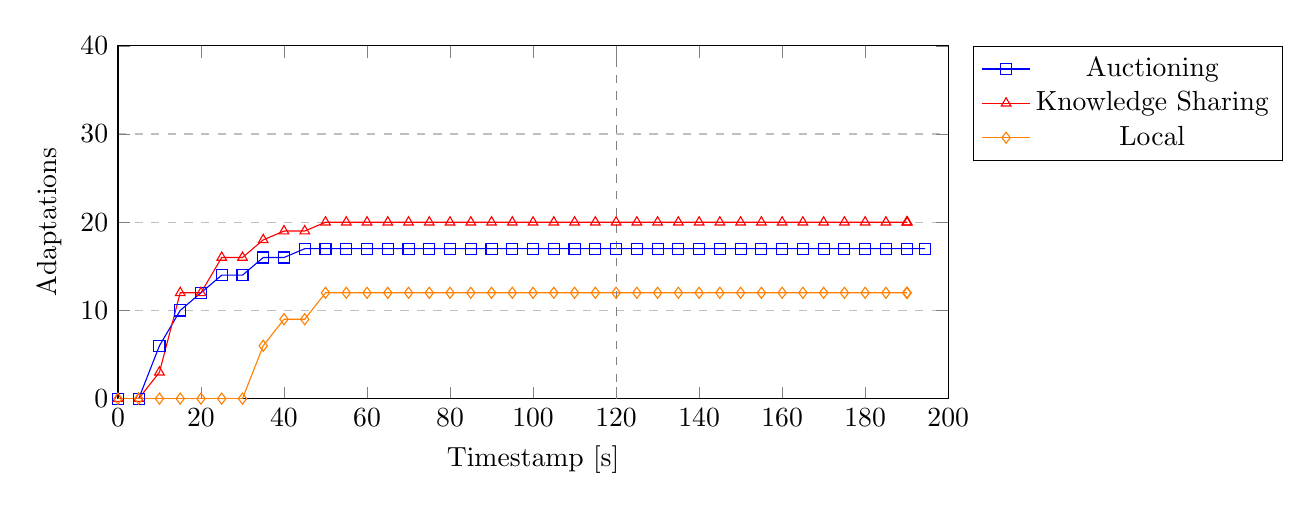
\begin{tikzpicture}
\begin{axis}[
    xlabel={Timestamp [s]},
    ylabel={Adaptations},
    xmin=0, xmax=200000,
    ymin=0, ymax=40,
    legend pos=outer north east,
    ymajorgrids=true,
    grid style=dashed,
    width=\textwidth,
    height=0.5\textwidth,
    scaled x ticks=base 10:-3,
    xtick scale label code/.code={}
]

	\addplot[color=blue,mark=square] coordinates {
        (0,0)(5000,0)(10000,6)(15000,10)(20000,12)(25000,14)(30000,14)(35000,16)(40000,16)(45000,17)(50000,17)(55000,17)(60000,17)(65000,17)(70000,17)(75000,17)(80000,17)(85000,17)(90000,17)(95000,17)(100000,17)(105000,17)(110000,17)(115000,17)(120000,17)(125000,17)(130000,17)(135000,17)(140000,17)(145000,17)(150000,17)(155000,17)(160000,17)(165000,17)(170000,17)(175000,17)(180000,17)(185000,17)(190000,17)(194444,17)
    };
    \addlegendentry{Auctioning}
	\addplot[color=red,mark=triangle] coordinates {
        (0,0)(5000,0)(10000,3)(15000,12)(20000,12)(25000,16)(30000,16)(35000,18)(40000,19)(45000,19)(50000,20)(55000,20)(60000,20)(65000,20)(70000,20)(75000,20)(80000,20)(85000,20)(90000,20)(95000,20)(100000,20)(105000,20)(110000,20)(115000,20)(120000,20)(125000,20)(130000,20)(135000,20)(140000,20)(145000,20)(150000,20)(155000,20)(160000,20)(165000,20)(170000,20)(175000,20)(180000,20)(185000,20)(190000,20)(190175,20)
    };
    \addlegendentry{Knowledge Sharing}
	\addplot[color=orange,mark=diamond] coordinates {
        (0,0)(5000,0)(10000,0)(15000,0)(20000,0)(25000,0)(30000,0)(35000,6)(40000,9)(45000,9)(50000,12)(55000,12)(60000,12)(65000,12)(70000,12)(75000,12)(80000,12)(85000,12)(90000,12)(95000,12)(100000,12)(105000,12)(110000,12)(115000,12)(120000,12)(125000,12)(130000,12)(135000,12)(140000,12)(145000,12)(150000,12)(155000,12)(160000,12)(165000,12)(170000,12)(175000,12)(180000,12)(185000,12)(190000,12)(190124,12)
    };
    \addlegendentry{Local}

	\addplot[color=gray, dashed,] coordinates {(120000,0) (120000,40)};


\end{axis}
\end{tikzpicture}
    \caption{Graph showing the total amount of adaptations applied by agents in the risk introduction scenario.}
    \label{fig:proposals-risk-introduction}
\end{figure}

When the risk is introduced after $120$ seconds, we can see in Figure \ref{fig:proposals-risk-introduction} that a few new adaptations are applied. This is in line with the damage graph in Figure \ref{fig:overall-damage-inroduce-risk}.

\begin{figure}[H]
    \centering
        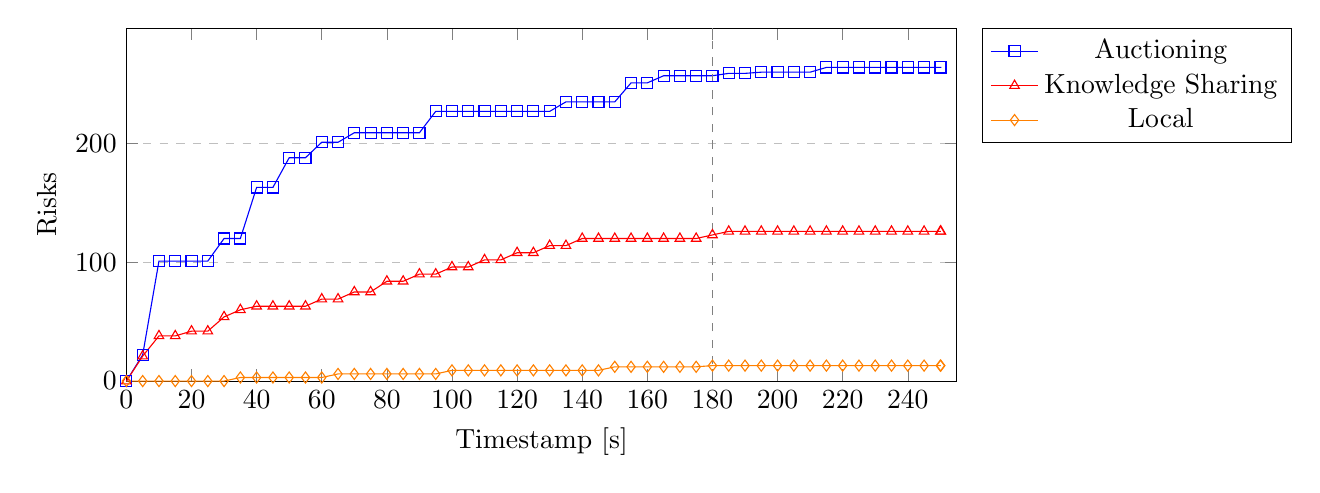
\begin{tikzpicture}
\begin{axis}[
    xlabel={Timestamp [s]},
    ylabel={Risks},
    xmin=0, xmax=255000,
    ymin=0, ymax=297,
    legend pos=outer north east,
    ymajorgrids=true,
    grid style=dashed,
    width=\textwidth,
    height=0.5\textwidth,
    scaled x ticks=base 10:-3,
    xtick scale label code/.code={}
]

	\addplot[color=blue,mark=square] coordinates {
        (0,0)(5000,22)(10000,101)(15000,101)(20000,101)(25000,101)(30000,120)(35000,120)(40000,163)(45000,163)(50000,188)(55000,188)(60000,201)(65000,201)(70000,209)(75000,209)(80000,209)(85000,209)(90000,209)(95000,227)(100000,227)(105000,227)(110000,227)(115000,227)(120000,227)(125000,227)(130000,227)(135000,235)(140000,235)(145000,235)(150000,235)(155000,251)(160000,251)(165000,257)(170000,257)(175000,257)(180000,257)(185000,259)(190000,259)(195000,260)(200000,260)(205000,260)(210000,260)(215000,264)(220000,264)(225000,264)(230000,264)(235000,264)(240000,264)(245000,264)(250000,264)(250288,264)
    };
    \addlegendentry{Auctioning}
	\addplot[color=red,mark=triangle] coordinates {
        (0,0)(5000,21)(10000,38)(15000,38)(20000,42)(25000,42)(30000,54)(35000,60)(40000,63)(45000,63)(50000,63)(55000,63)(60000,69)(65000,69)(70000,75)(75000,75)(80000,84)(85000,84)(90000,90)(95000,90)(100000,96)(105000,96)(110000,102)(115000,102)(120000,108)(125000,108)(130000,114)(135000,114)(140000,120)(145000,120)(150000,120)(155000,120)(160000,120)(165000,120)(170000,120)(175000,120)(180000,123)(185000,126)(190000,126)(195000,126)(200000,126)(205000,126)(210000,126)(215000,126)(220000,126)(225000,126)(230000,126)(235000,126)(240000,126)(245000,126)(250000,126)(250159,126)
    };
    \addlegendentry{Knowledge Sharing}
	\addplot[color=orange,mark=diamond] coordinates {
        (0,0)(5000,0)(10000,0)(15000,0)(20000,0)(25000,0)(30000,0)(35000,3)(40000,3)(45000,3)(50000,3)(55000,3)(60000,3)(65000,6)(70000,6)(75000,6)(80000,6)(85000,6)(90000,6)(95000,6)(100000,9)(105000,9)(110000,9)(115000,9)(120000,9)(125000,9)(130000,9)(135000,9)(140000,9)(145000,9)(150000,12)(155000,12)(160000,12)(165000,12)(170000,12)(175000,12)(180000,13)(185000,13)(190000,13)(195000,13)(200000,13)(205000,13)(210000,13)(215000,13)(220000,13)(225000,13)(230000,13)(235000,13)(240000,13)(245000,13)(250000,13)(250135,13)
    };
    \addlegendentry{Local}

	\addplot[color=gray, dashed,] coordinates {(180000,0) (180000,297)};


\end{axis}
\end{tikzpicture}
    \caption{Graph showing the number of unique risks detected by agents in the risk introduction scenario.}
    \label{fig:risk-count-risk-introduction}
\end{figure}

When we look at Figure \ref{fig:risk-count-risk-introduction} we can see that the knowledge-sharing agent detects the most risks, followed by the auctioning agent. The local-agent detects the least amount of risks, at only $10\%$ of the risks found by the knowledge-sharing agent. We would expect a comparable result between the auctioning and knowledge-sharing agents, however this is not the case. This is likely due to the fact that in the knowledge-sharing setup agents apply multiple adaptations in parallel. This causes the knowledge bases to change more rapidly, which could cause the agents to detect more risks. This is explained in more detail in subsection \ref{ssec:metrics}.

\begin{figure}[H]
    \centering
        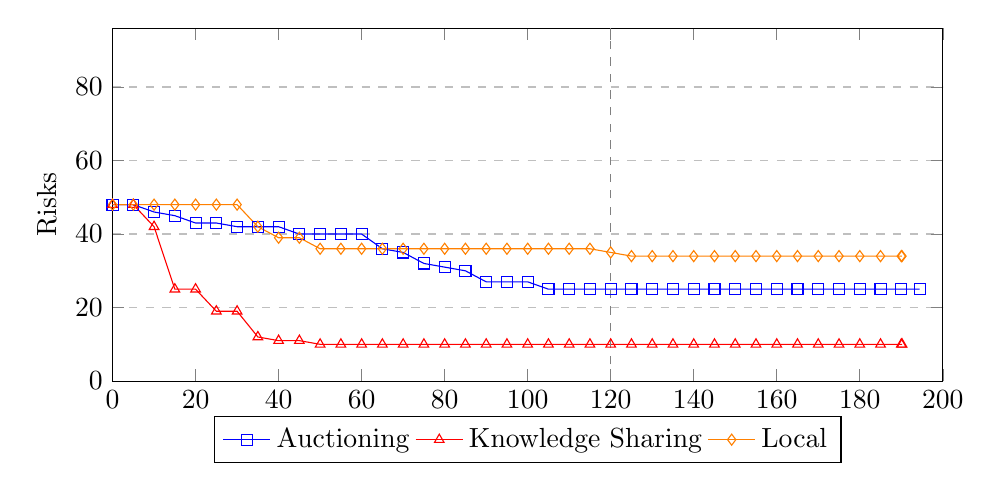
\begin{tikzpicture}
\begin{axis}[
    xlabel={Timestamp [s]},
    ylabel={Risks},
    xmin=0, xmax=200000,
    ymin=0, ymax=96,
    legend columns=-1,
    legend style={at={(0.5,-0.1)},anchor=north},
    ymajorgrids=true,
    grid style=dashed,
    width=\textwidth,
    height=0.5\textwidth,
    scaled x ticks=base 10:-3,
    xtick scale label code/.code={}
]

	\addplot[color=blue,mark=square] coordinates {
        (0,48)(5000,48)(10000,46)(15000,45)(20000,43)(25000,43)(30000,42)(35000,42)(40000,42)(45000,40)(50000,40)(55000,40)(60000,40)(65000,36)(70000,35)(75000,32)(80000,31)(85000,30)(90000,27)(95000,27)(100000,27)(105000,25)(110000,25)(115000,25)(120000,25)(125000,25)(130000,25)(135000,25)(140000,25)(145000,25)(150000,25)(155000,25)(160000,25)(165000,25)(170000,25)(175000,25)(180000,25)(185000,25)(190000,25)(194440,25)
    };
    \addlegendentry{Auctioning}
	\addplot[color=red,mark=triangle] coordinates {
        (0,48)(5000,48)(10000,42)(15000,25)(20000,25)(25000,19)(30000,19)(35000,12)(40000,11)(45000,11)(50000,10)(55000,10)(60000,10)(65000,10)(70000,10)(75000,10)(80000,10)(85000,10)(90000,10)(95000,10)(100000,10)(105000,10)(110000,10)(115000,10)(120000,10)(125000,10)(130000,10)(135000,10)(140000,10)(145000,10)(150000,10)(155000,10)(160000,10)(165000,10)(170000,10)(175000,10)(180000,10)(185000,10)(190000,10)(190192,10)
    };
    \addlegendentry{Knowledge Sharing}
	\addplot[color=orange,mark=diamond] coordinates {
        (0,48)(5000,48)(10000,48)(15000,48)(20000,48)(25000,48)(30000,48)(35000,42)(40000,39)(45000,39)(50000,36)(55000,36)(60000,36)(65000,36)(70000,36)(75000,36)(80000,36)(85000,36)(90000,36)(95000,36)(100000,36)(105000,36)(110000,36)(115000,36)(120000,35)(125000,34)(130000,34)(135000,34)(140000,34)(145000,34)(150000,34)(155000,34)(160000,34)(165000,34)(170000,34)(175000,34)(180000,34)(185000,34)(190000,34)(190162,34)
    };
    \addlegendentry{Local}

	\addplot[color=gray, dashed,] coordinates {(120000,0) (120000,96)};


\end{axis}
\end{tikzpicture}
    \caption{Graph showing the number of remaining risks in the infrastructure in the risk introduction scenario.}
    \label{fig:risk-remaining-risk-introduction}
\end{figure}

\add{Write}

\begin{figure}[H]
    \hspace*{-1cm}
    \centering
        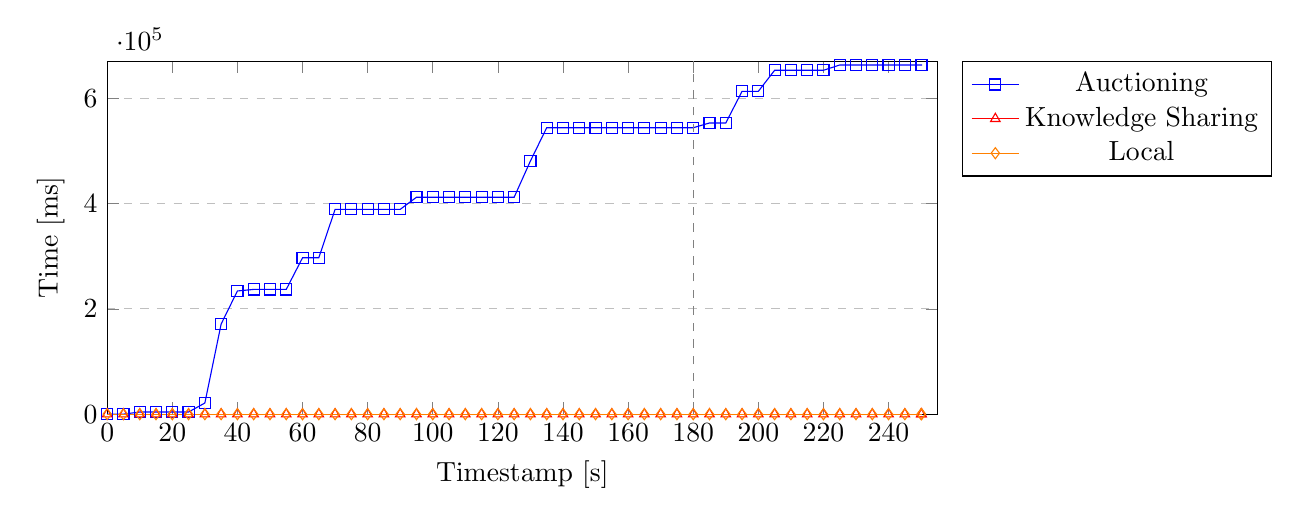
\begin{tikzpicture}
\begin{axis}[
    xlabel={Timestamp [s]},
    ylabel={Time [ms]},
    xmin=0, xmax=255000,
    ymin=0, ymax=670067,
    legend pos=outer north east,
    ymajorgrids=true,
    grid style=dashed,
    width=\textwidth,
    height=0.5\textwidth,
    scaled x ticks=base 10:-3,
    xtick scale label code/.code={}
]

	\addplot[color=blue,mark=square] coordinates {
        (0,0)(5000,64)(10000,4143)(15000,4143)(20000,4143)(25000,4143)(30000,21179)(35000,171183)(40000,233978)(45000,236929)(50000,236929)(55000,236929)(60000,297046)(65000,297049)(70000,388980)(75000,388980)(80000,388980)(85000,388980)(90000,388980)(95000,411980)(100000,411980)(105000,411980)(110000,411980)(115000,411980)(120000,411980)(125000,411980)(130000,480905)(135000,543951)(140000,543951)(145000,543951)(150000,543951)(155000,543958)(160000,543958)(165000,543962)(170000,543962)(175000,543962)(180000,543962)(185000,553054)(190000,553054)(195000,613073)(200000,613073)(205000,653079)(210000,653079)(215000,653087)(220000,653087)(225000,663101)(230000,663101)(235000,663101)(240000,663101)(245000,663101)(250000,663101)(250288,663101)
    };
    \addlegendentry{Auctioning}
	\addplot[color=red,mark=triangle] coordinates {
        (0,0)(5000,0)(10000,0)(15000,0)(20000,0)(25000,0)(30000,0)(35000,0)(40000,0)(45000,0)(50000,0)(55000,0)(60000,0)(65000,0)(70000,0)(75000,0)(80000,0)(85000,0)(90000,0)(95000,0)(100000,0)(105000,0)(110000,0)(115000,0)(120000,0)(125000,0)(130000,0)(135000,0)(140000,0)(145000,0)(150000,0)(155000,0)(160000,0)(165000,0)(170000,0)(175000,0)(180000,0)(185000,0)(190000,0)(195000,0)(200000,0)(205000,0)(210000,0)(215000,0)(220000,0)(225000,0)(230000,0)(235000,0)(240000,0)(245000,0)(250000,0)(250159,0)
    };
    \addlegendentry{Knowledge Sharing}
	\addplot[color=orange,mark=diamond] coordinates {
        (0,0)(5000,0)(10000,0)(15000,0)(20000,0)(25000,0)(30000,0)(35000,0)(40000,0)(45000,0)(50000,0)(55000,0)(60000,0)(65000,0)(70000,0)(75000,0)(80000,0)(85000,0)(90000,0)(95000,0)(100000,0)(105000,0)(110000,0)(115000,0)(120000,0)(125000,0)(130000,0)(135000,0)(140000,0)(145000,0)(150000,0)(155000,0)(160000,0)(165000,0)(170000,0)(175000,0)(180000,0)(185000,0)(190000,0)(195000,0)(200000,0)(205000,0)(210000,0)(215000,0)(220000,0)(225000,0)(230000,0)(235000,0)(240000,0)(245000,0)(250000,0)(250135,0)
    };
    \addlegendentry{Local}

	\addplot[color=gray, dashed,] coordinates {(180000,0) (180000,670067)};


\end{axis}
\end{tikzpicture}
    \caption{Graph showing the sum of time spent auctioning by agents in the risk introduction scenario.}
    \label{fig:auctioning-time-risk-introduction}
\end{figure}

As with Figure \ref{fig:auctioning-time-no-change}, we see in Figure \ref{fig:adapting-time-risk-introduction} that only the auctioning agent spends time auctioning. The knowledge-sharing agent spends no time auctioning, as it does not have this feature-set. After the $120$ seconds mark we see that the auctioning agent spends more time auctioning, which is a result of the risk being introduced.

\begin{figure}[H]
    \hspace*{-1cm}
    \centering
        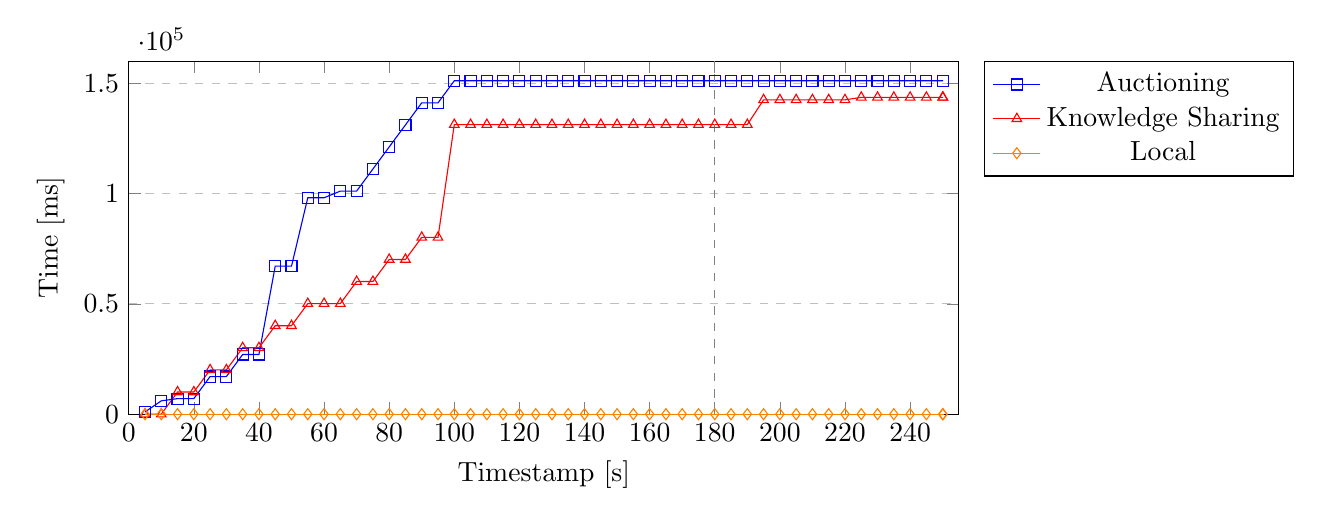
\begin{tikzpicture}
\begin{axis}[
    xlabel={Timestamp [s]},
    ylabel={Time [ms]},
    xmin=0, xmax=255000,
    ymin=0, ymax=160016,
    legend pos=outer north east,
    ymajorgrids=true,
    grid style=dashed,
    width=\textwidth,
    height=0.5\textwidth,
    scaled x ticks=base 10:-3,
    xtick scale label code/.code={}
]

	\addplot[color=blue,mark=square] coordinates {
        (5000,1002)(10000,6043)(15000,7052)(20000,7052)(25000,17062)(30000,17062)(35000,27073)(40000,27073)(45000,67114)(50000,67114)(55000,98143)(60000,98143)(65000,101166)(70000,101166)(75000,111175)(80000,121177)(85000,131184)(90000,141191)(95000,141191)(100000,151201)(105000,151201)(110000,151201)(115000,151201)(120000,151201)(125000,151201)(130000,151201)(135000,151201)(140000,151201)(145000,151201)(150000,151201)(155000,151201)(160000,151201)(165000,151201)(170000,151201)(175000,151201)(180000,151201)(185000,151201)(190000,151201)(195000,151201)(200000,151201)(205000,151201)(210000,151201)(215000,151201)(220000,151201)(225000,151201)(230000,151201)(235000,151201)(240000,151201)(245000,151201)(250000,151201)(250139,151201)
    };
    \addlegendentry{Auctioning}
	\addplot[color=red,mark=triangle] coordinates {
        (5000,0)(10000,0)(15000,10047)(20000,10047)(25000,20080)(30000,20080)(35000,30102)(40000,30102)(45000,40126)(50000,40126)(55000,50144)(60000,50144)(65000,50144)(70000,60152)(75000,60152)(80000,70161)(85000,70161)(90000,80163)(95000,80163)(100000,131322)(105000,131322)(110000,131322)(115000,131322)(120000,131322)(125000,131322)(130000,131322)(135000,131322)(140000,131322)(145000,131322)(150000,131322)(155000,131322)(160000,131322)(165000,131322)(170000,131322)(175000,131322)(180000,131322)(185000,131322)(190000,131322)(195000,142557)(200000,142557)(205000,142557)(210000,142557)(215000,142557)(220000,142557)(225000,143673)(230000,143673)(235000,143673)(240000,143673)(245000,143673)(250000,143673)(250111,143673)
    };
    \addlegendentry{Knowledge Sharing}
	\addplot[color=orange,mark=diamond] coordinates {
        (5000,0)(10000,0)(15000,0)(20000,0)(25000,0)(30000,0)(35000,0)(40000,0)(45000,0)(50000,0)(55000,0)(60000,0)(65000,0)(70000,0)(75000,0)(80000,0)(85000,0)(90000,0)(95000,0)(100000,0)(105000,0)(110000,0)(115000,0)(120000,0)(125000,0)(130000,0)(135000,0)(140000,0)(145000,0)(150000,0)(155000,0)(160000,0)(165000,0)(170000,0)(175000,0)(180000,0)(185000,0)(190000,0)(195000,0)(200000,0)(205000,0)(210000,0)(215000,0)(220000,0)(225000,0)(230000,0)(235000,0)(240000,0)(245000,0)(250000,0)(250115,0)
    };
    \addlegendentry{Local}

	\addplot[color=gray, dashed,] coordinates {(180000,0) (180000,160016)};


\end{axis}
\end{tikzpicture}
    \caption{Graph showing the sum of time spent adapting by agents in the risk introduction scenario.}
    \label{fig:adapting-time-risk-introduction}
\end{figure}

Figure \ref{fig:adapting-time-risk-introduction} shows that the knowledge-sharing agent is still spending more time adapting compared to the auctioning agent. Compared to Figure \ref{fig:adapting-time-no-change} we see that the agents are all spending roughly the same amount of time adapting, until the $120$ second mark. After this time a bump is observable in the graph.
